\documentclass[letterpaper,notitlepage,twoside]{article}

% Basic imports, increase margins...
\usepackage[margin=0.75in]{geometry}
\usepackage{amssymb}
\usepackage{amsmath}

% Finite State Machine stuff
\usepackage{pgf}
\usepackage{tikz}
\usetikzlibrary{arrows,automata}
\usepackage{pgfplots}

% Format tables nicely
\usepackage[latin1]{inputenc}
\usepackage{array}
\usepackage{booktabs}
\setlength{\heavyrulewidth}{1.5pt}
\setlength{\abovetopsep}{4pt}

\usepackage{amsfonts} 
\usepackage{amssymb}
\usepackage{amsmath,amsthm}

\renewcommand{\implies}{\Rightarrow} % redefine command "implies"  
\renewcommand{\iff}{\Leftrightarrow} % double arrow
\newcommand{\maps}{\rightarrow} % define command "map" 
\newcommand{\union}{\cup}
\newcommand{\intersect}{\cap}
\newcommand{\N}{\mathbb{N}} % natural number 
\newcommand{\Q}{\mathbb{Q}} % rational number 
\newcommand{\R}{\mathbb{R}} % real number 
\newcommand{\Z}{\mathbb{Z}} % integers 
\newcommand\tab[1][1cm]{\hspace*{#1}} %\tab command

% Add more packages that you use here..

\title{CS 1510 Homework 2}
\author{Brian Falkenstein, Brian Knotten, Brett Schreiber}

\begin{document}
\maketitle

\section*{4}
\subsection*{a}
\begin{itemize}
	\item Let $A$ be an algorithm which produces a list fill amounts a motorist takes at each stop. 
	\item For sake of contradiction assume $A$ is not correct.
	\item Therefore there exists an input $I$ where $A$ produces a non-optimal output.
	\item Let $opt(I)$ be the optimal output that differs the least from $A(I)$.
	\item Since $A(I) \neq opt(I)$, there exists a first item in the list at stop $x_i$ where $A(I)$'s fill amount $f$ differs from $opt(I)$'s fill amount $g$.
	\item Every prior fill amount before $x_i$ must be identical between $A(I)$ and $opt(I)$.
	\item Since $f \neq g$, then $f > g$ or $f < g$.
	\item If $f > g$:
	\begin{itemize}
		\item Since $opt(I)$ is correct, $g$ was enough fuel to get to the next stop.
		\item Therefore $f$ was not the minimum amount of gas needed.
		\item $A$ guarantees only filling up the minimum amount of gas needed.
		\item There is a contradiction.
	\end{itemize}
	
	\item So it can only be the case that $f < g$.
	\item $A(I)$ spends less time ( $\frac{g - f}{r}$ seconds) filling up at $x_i$.
	\item Since $A(I)$ is correct (yet suboptimal), $f$ was enough fuel to get to the next stop.
	\item Consider an alternative optimal solution $opt'(I)$ identical to $opt(I)$ except fill amount $g$ is replaced with $f$ at $x_i$.
	\item The time is still optimal, since less time is spent fueling at $x_i$. ($\frac{g - f}{r}$) seconds less.
	\item $opt'(I)$ cannot use less time than $opt(I)$, otherwise $opt(I)$ would not be optimal. So $opt'(I)$ utilizes $\frac{g - f}{r}$ seconds somewhere else.
	\item This extra time can be used to ensure that $opt'(I)$ is still a correct algorithm.
\end{itemize}


\subsection*{b}
This algorithm $A$ does not provide an optimal output for the following input $I$:\\
\begin{itemize}
	\item Let $A$ be the first gas station at kilometer 0
	\item Let $x$ be the second gas station at kilometer 2
	\item Let $B$ be the destination at kilometer 4
	\item Let $C$ be the capacity 3 liters
	\item Let $F$ be the consumption rate of 1 liter per kilometer
	\item Let $r$ be the fill rate of 1 liter per minute
\end{itemize}
$A(I)$ produces the following output (a list of actions):
\begin{enumerate}
	\item Fuel tank starts at 0/3.
	\item Not enough gas to make it to $x$, so fill the tank up all the way with 3 liters at $A$, taking 3 minutes. (Fuel tank at 3/3).
	\item Travel to gas station $x$, 2 kilometers away. (Fuel tank at 1/3).
	\item Not enough gas to make it to $B$, so fill the tank up all the way with 2 liters at $x$ taking 2 minutes. (Fuel tank at 3/3).
	\item Arrive at destination $B$, 2 kilometers away. (Fuel tank at 1/3).
\end{enumerate}
$A(I)$ requires 3 + 2 = 5 minutes of fueling.

A better output $O(I)$ is:
\begin{enumerate}
	\item Fuel tank starts at 0/3.
	\item Fill 3 liters at $A$, taking 3 minutes. (Fuel tank at 3/3).
	\item Travel to gas station $x$, 2 kilometers away. (Fuel tank at 1/3).
	\item Fill 1 liters at $x$, taking 1 minute. (Fuel tank at 1/3).
	\item Arrive at destination $B$, 2 kilometers away. (Fuel tank at 0/3).
\end{enumerate}
$O(I)$ requires 3 + 1 = 4 minutes of fueling.\\

Since there exists a more optimal output than $A(I)$, $A$ is not a correct algorithm.
\section*{5}
\subsection*{a}
The presented algorithm (hereafter referred to as $A$) is not correct as it does not provide an optimal output for the presented problem for the following input (hereafter referred to as $P$). For the sake of simplicity I will be presenting the input ($P$) as a list of points on the real line and the unit intervals as intervals of length 1 on the real line. Additionally, $S$ shall be the solution set of intervals.
\begin{itemize}
	\item Let $P = \{1, 1.6, 1.7, 1.8, 2.1, 2.2, 2.9, 2.95, 3.3, 3.4, 3.5, 4 \}$ \\\\
	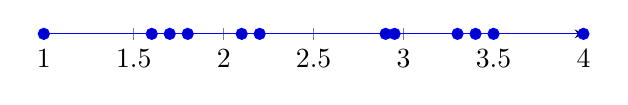
\begin{tikzpicture}
        \begin{axis}[
            axis x line=middle,
            axis y line=none,
            height=50pt,
            width=\axisdefaultwidth,
            xmin=1,
            xmax=4,
        ]
            \addplot coordinates {
                (1,0) (1.6,0) (1.7,0) (1.8,0) (2.1,0) (2.2,0) (2.9,0) (2.95,0) (3.3,0) (3.4,0) (3.5,0) (4,0)
            };
        \end{axis}
    \end{tikzpicture}
    \item $A$ always selects the interval that covers the most points; clearly, the intervals from from 1.6 to 2.2 and from 2.9 to 3.5 cover the most points as they both cover 5 points each. For the sake of argument, let's say $A$ selects the interval from 1.6 to 2.2 first and adds it to $S$.
    \item $A$ will next select the interval from 2.9 and 3.5 and add it to $S$ as it also covers 5 points.
    \item $A$ is now left with points 1 and 4 to cover with intervals. They will have to be covered separately, as they are more than 1 unit away from each other.
    \item After covering 1 and 4, $A$'s optimal output is: $P = \{1, \ $1.6-2.2, 2.9-3.5$ \ , 4 \}$
    \item However, a more optimal output is the obvious three intervals from 1-2, 2-3, and 3-4.
    \item Since there exists a more optimal output than $A(P)$, $A$ is not a correct algorithm.
	
\end{itemize}

\subsection*{b}
This algorithm $A$ solves the problem. Because I am using $A$ to refer to the algorithm, I will refer to the set of points listed in the problem as $P$. 
\begin{itemize}
	\item Assume the algorithm $A$ is incorrect, and has some input $I$ that causes it to give suboptimal output. 
	\item Let $O(I)$ be the optimal algorithm on $I$ that differs the least from $A(I)$. 
	\item Let $j$ be the first point that the algorithms differ. That is, before we've reached $p_j$, the $j'th$ item in $P$, $A(I)=O(I)$. 
	\item Because of our assumption, $O(I)$ chose another way of covering point $p_j$ with a unit interval. Because we know that $A(I)$ will have a unit interval beginning at point $p_j$, by definition of the algorithm, that leaves 2 possibilities for how $O(I)$ placed the unit interval. 
	\item Either $O(I)$ has a unit interval ending at point $p_j$, or $O(I)$ placed a unit interval, where $p_j$ appears somewhere in between. 
	\item Neither of these situations are more optimal than the one $A$ chose. 
	\item In the case that the interval ends at $p_j$, we know that it is not more optimal, as if it covered more points before $p_j$, $A$ would have already selected one of those earlier points, placing a unit interval beginning at one of those points and covering $p_j$. 
	\item Similarly, in the case that $p_j$ appears somewhere in the middle of the interval placed by $O$, no points appearing earlier would be captured (for the reason stated above), and any point after $p_j$ that would be captured by this interval would also be captured by the interval that $A$ placed.
	\item Thus, we can construct $O'(I)$ by removing the interval it placed at step j, and adding an interval beginning at $p_j$. 
	\item $O'(I)$ agrees with $A(I)$ for one more step without sacrificing correctness, so we have reached a contradiction. 
\end{itemize}	
\end{document}
